\documentclass[a4paper]{article}

\usepackage[english]{babel}
\usepackage[utf8x]{inputenc}
\usepackage[T1]{fontenc}

\usepackage[a4paper,top=3cm,bottom=2cm,left=3cm,right=3cm,marginparwidth=1.75cm]{geometry}

\usepackage{nth}
\usepackage{amsmath}
\usepackage{graphicx}
\usepackage[hidelinks]{hyperref}
\usepackage{enumitem}

\usepackage{parskip}
\usepackage{lscape}
\usepackage{pdfpages}

\newcommand{\ts}{\textsuperscript}
%TODO: Check all paging and add breaks where appropriate.
\title{\vspace{-2cm}Integrated Group Project}
\author{NA3
	\\ \rule{5cm}{0.4pt}
	\\Adam Howes - 00000000,
	\\Ben Ashing - 15846150,
	\\Charlie Howes - 15823951,
	\\Constantinos Ioannou - 00000000,
	\\Lewis Allen - 15816594,
    \\ \rule{5cm}{0.4pt}
} %TODO: Look at making the rule closer to the text.

\begin{document}
\maketitle

\tableofcontents

\break

\section{Preface}
Throughout this document we refer to the following group members using their initials in individual sections:
\begin{itemize}
    \item Adam Howes (AH) - Configuration Manager 
    \item Ben Ashing (BA) - Project Leader
    \item Charlie Howes (CH) - Technical Leader
    \item Constantinos Ioannou (CI) - Process Leader
    \item Lewis Allen (LA) - Quality Assurance
\end{itemize}


\begin{landscape} %TODO: Look at making this nicer somehow
\section{Planning}
\subsection{Gantt Chart}
\subsubsection{Proposed}
\begin{figure}[!ht] %TODO: Maybe make this landscape, would be easier to read.
    \centering
    \makebox[0.75\textwidth]{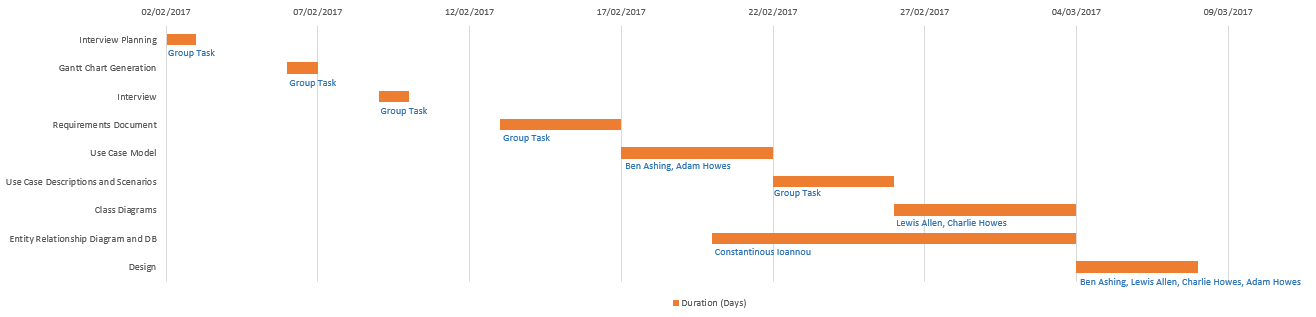
\includegraphics[width=0.75\paperheight]{ProposedGanttChart.png}} %TODO: Check this sizing at the end.
    \caption{Proposed Gantt Chart}
    \label{fig:proposed_gantt}
\end{figure}

\clearpage
\subsubsection{Actual} %TODO: This might be better at the end, but not 100% sure.
\begin{figure}[!ht]
    \centering
    \makebox[0.75\textwidth]{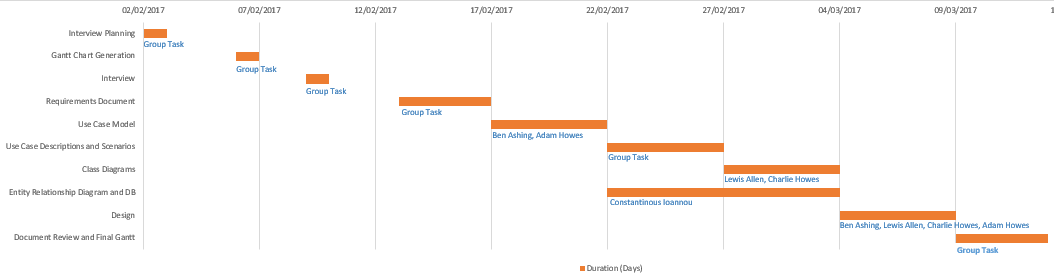
\includegraphics[width=0.75\paperheight]{ActualGanttChart.png}} %TODO: Check this sizing at the end.
    \caption{Actual Gantt Chart}
    \label{fig:actual_gantt}
\end{figure}
\end{landscape}

\subsection{Minutes} %TODO: Fill this in from github

\section{Requirements}

\subsection{Document} %TODO: Need to rename one of these.

\begin{enumerate}
  \item Business Requirements
  \begin{enumerate}[label=B\arabic*.]
    \item The Planning should be completed by March \nth{13}
    \item The finished product should be delivered in May.
    \item The software will be adopted and used by all staff.
  \end{enumerate}

  \item User Requirements
  \begin{enumerate}[label=U\arabic*.] 
    \item Users must be able to log in using a user name and password.
    \item Users must be able to log out
    \item The user must be able to personalize their view.
    \item The user must able to easily view calendars for daily, monthly and yearly schedules.
    \item The user must be able to set recurring appointments.
    \item Staff must be able to create groups.
    \item Staff must be able to modify groups
    \item Staff must be able to add other staff/groups to events.
    \item The user must be able to cancel appointments at any time within a session.
    \item The user must be able to use a search feature to find other users.
    \item The user should be able to make event requests. 
    \begin{enumerate}[label*=\arabic*.]
      \item Users should be able to receive event requests.
      \item Users should be able to accept event requests.
      \item Users should be able to decline event requests.
    \end{enumerate}
  \end{enumerate}

  \item Quality Requirements
  \begin{enumerate}[label=Q\arabic*.]
    \item The application must use symbols to clearly show changes in events.
    \item The application should notify the user in any changes to events such as cancellations.
    \item The application must implement optimized loading times.
  \end{enumerate}
  \item Functional Requirements
  \begin{enumerate}[label=F\arabic*.]
    \item Only members of staff should be assigned accounts.
    \item The architecture of the project should support different platforms.
    \item A method must exist which allows staff to be given administration rights to form an administrative team.
    \item Administrators must be able to verify accounts.
  \end{enumerate}
  \item Non-Functional Requirements
  \begin{enumerate}[label=NF\arabic*.]
  	  \item The user should be able to complete any single task with a minimum of eight actions. (LA)
      \item The code needs to be easily maintainable by keeping the code organized, well written, documented and simple. (CH)
      \item The project must be easily scaled to implement additional features and a larger user base. (CH) %TODO: Be more specific with numbers
      \item The program must be executable on the following Operating Systems: (AH) \begin{itemize}
        \item Windows 8, 8.1 \& 10
        \item Mac OS
        \item Linux Ubuntu
      \end{itemize}
      \item The minimum specifications to run the program should be: (AH) \begin{itemize}
        \item Processor: Pentium 4
        \item RAM: 500MB
        \item Disk Space: 100MB
      \end{itemize}
      \item The code must also be able to run on both 32 and 64-bit Operating Systems and be able to view events when not connected to the Internet. (AH)
      \item All personal data must be fully secure through encryption and hashing. (BA)
      \item The project must be adaptable in the future for mobile implementations. (CI)
  \end{enumerate}
\end{enumerate}

\clearpage % Forces the figure to be in this subsection by clearing the floats.
\subsection{Stakeholder Diagram}

\begin{figure}[!ht]
    \centering
    \makebox[0.75\textwidth]{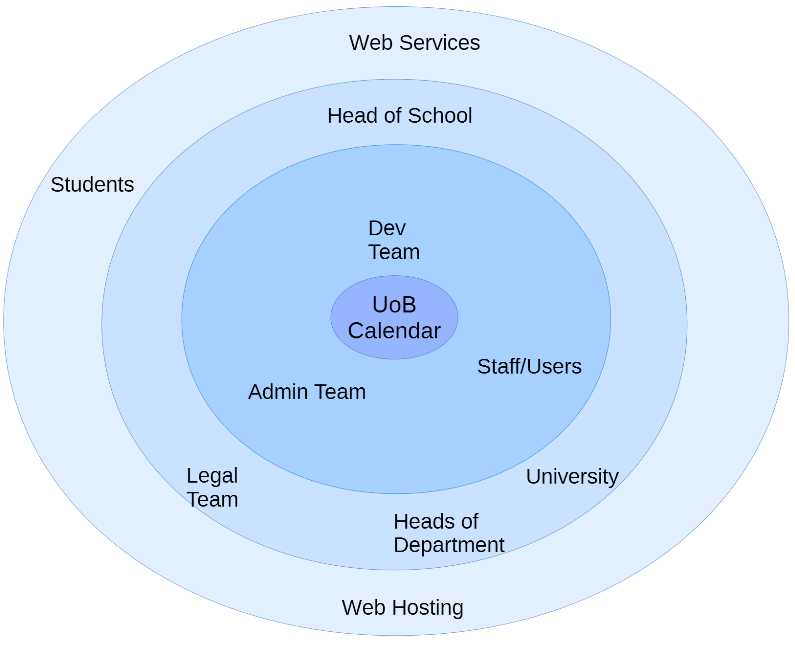
\includegraphics[width=0.75\paperwidth]{OnionModel.png}} %TODO: Check this sizing at the end.
    \caption{Stakeholder Diagram}
    \label{fig:stakeholder}
\end{figure}

\clearpage
\section{Use Case Model}
\begin{figure}[!ht] %TODO: Look into making this landscape too
    \centering\makebox[0.9\textwidth]{\includegraphics[width=0.75\paperwidth]{UseCase.jpg}} %TODO: Check this sizing at the end.
    \caption{Use Case Diagram}
    \label{fig:usecase}
\end{figure}

\subsection{Case Descriptions} %TODO: Add other descriptions when they are done alongside screens.
\subsubsection{Login - CI}
\underline{\textit{Use case}}: Login

\underline{\textit{Actors}}: User (Primary)

\underline{\textit{Precondition}}: Time, Date \& Location from customer (via phone).

\underline{\textit{Success postcondition}}: The user fills in their login credentials successfuly and logs into the system.

\underline{\textit{Failure postcondition}}: The user does not fill the correct login credentials.

\underline{\textit{Trigger}}: The personal calendar of the user is displayed

\underline{\textit{Main success scenario}}: 
\begin{enumerate}[leftmargin = 3em]
    \item User wants to login
    \item User inserts credentials into the system
    \item User clicks the login button
    \item System checks the input credentials.
    \item System fetches information and displays their personal calendar
\end{enumerate} 

\underline{\textit{Extensions}}:
\begin{enumerate}[label=3\alph*, leftmargin = 3em]
    \item User entered invalid data \begin{enumerate}[label=\arabic*.]
        \item System asks the user to input correct data
        \item Restart from 2
    \end{enumerate}
\end{enumerate}

\subsubsection{Creating an Event - LA}
\underline{\textit{Use case}}: Creating an Event

\underline{\textit{Actors}}: User (Primary)

\underline{\textit{Precondition}}: The User has logged into their account.

\underline{\textit{Success postcondition}}: The User has the created event displayed on their calendar.

\underline{\textit{Failure postcondition}}: The User was unable to create the event.

\underline{\textit{Trigger}}: The User clicks the ‘add event’ button.

\underline{\textit{Main success scenario}}: 
\begin{enumerate}[leftmargin = 3em]
    \item The user clicks the ‘add event’ button.
    \item The User specifies the time, day and duration of the event.
    \item The user names the event and gives it a description.
    \item The user clicks ‘Confirm’.
    \item The System adds the event to the user’s calendar.
\end{enumerate} 

\underline{\textit{Extensions}}:
\begin{enumerate}[label=2\alph*, leftmargin = 3em]
    \item The user has input an event time/date and there is a conflicting schedule. (The user already has an event booked for that duration) \begin{enumerate}[label=\arabic*.]
        \item The System indicates that the user can no longer click confirm.
        \item The System informs the user that there is already an event planned for that duration.
        \item The user is returned to the event creation screen and is given the option to change to event time/day, along with the other details if required.
        \item The user modifies the time/day to a free period.
        \item Continue on to step 3.
    \end{enumerate}
\end{enumerate}

\subsubsection{Edit Event - BA}
\underline{\textit{Use case}}: Editing the Details of Events

\underline{\textit{Actors}}: User (Primary)

\underline{\textit{Precondition}}: The user is logged in and has an event to edit.

\underline{\textit{Success postcondition}}: The User has successfully edited the details of their event.

\underline{\textit{Failure postcondition}}: The User is unable to edit the details of their event

\underline{\textit{Trigger}}: The User clicks on the event edit button.


\underline{\textit{Main success scenario}}: 
\begin{enumerate}[leftmargin = 3em]
    \item The User will navigate to the event in the calendar
    \item The User will select the event they wish to edit
    \item The User will click on the edit button
    \item The User will be able to change any detail of the even
    \item The User will click on the save button to save any changes
\end{enumerate} 

\underline{\textit{Extensions}}:
\begin{enumerate}[label=3\alph*, leftmargin = 3em]
    \item The User is not the host of the event \begin{enumerate}[label=\arabic*.]
        \item An edit button won’t be displayed to the user if they don’t have the right change it
    \end{enumerate}
\end{enumerate}

\begin{enumerate}[label=4\alph*, leftmargin = 3em]
    \item The User makes an illegal change to the event e.g. changing the date to a date in the past \begin{enumerate}[label=\arabic*.]
        \item The User is notified that the changes made cannot be saved
        \item The User Changes the data so that it is valid
        \item Proceed to step 5
    \end{enumerate}
\end{enumerate}

\begin{enumerate}[label=5\alph*, leftmargin = 3em]
    \item The User closes the calendar without saving the changes that have been made 
    \begin{enumerate}[label=\arabic*.]
        \item The User is notified that changes won’t be saved
        \begin{enumerate}[label=\alph*]
            \item \begin{enumerate}[label=\arabic*.]
                \item The user clicks cancel
                \item Proceed to step 5
            \end{enumerate}
            \item \begin{enumerate}[label=\arabic*.]
                \item The user ignores the notification and navigates away from the page
                \item Failure postcondition is met
            \end{enumerate}
        \end{enumerate}
    \end{enumerate}
\end{enumerate}

\subsubsection{Creating a Group - CH}
\underline{\textit{Use case}}: Creating a Group

\underline{\textit{Actors}}: User (Primary)

\underline{\textit{Precondition}}: The User has logged into their account.

\underline{\textit{Success postcondition}}: The User creates a group to use in events.

\underline{\textit{Failure postcondition}}: The User was unable to create a group

\underline{\textit{Trigger}}: The User clicks the "Add Group" button.

\underline{\textit{Main success scenario}}: 
\begin{enumerate}[leftmargin = 3em]
    \item The User inputs the name of the group
    \item The User inputs the description of the group
    \item The User clicks on the "Add Member" button and adds a member.
    \item The User clicks "Create".
    \item The System adds the group to the user.
\end{enumerate} 

\underline{\textit{Extensions}}:
\begin{enumerate}[label=1\alph*, leftmargin = 3em]
    \item The user didn't input the name of the group \begin{enumerate}[label=\arabic*.]
        \item The program disabled the "Create" button
        \item The user is informed that they are required to input a name.
        \begin{enumerate}[label=\alph*]
            \item The user clicks cancel \begin{enumerate}[label=\arabic*.]
                \item The program goes back to the previous screen.
                \item The failure postcondition is met.
            \end{enumerate}
            \item The user inputs the name \begin{enumerate}[label=\arabic*.]
                \item The program enables the "Create" button
                \item Continue from step 2. 
            \end{enumerate}
        \end{enumerate}
    \end{enumerate}
\end{enumerate}

\begin{enumerate}[label=4\alph*, leftmargin = 3em]
    \item The user clicks "Cancel" \begin{enumerate}[label=\arabic*.]
    \item The program goes back to the previous screen.
        \item The failure postcondition is met 
    \end{enumerate}
\end{enumerate}

\clearpage
\section{Class Diagram}
\subsection{Diagram}
\begin{figure}[!ht]
    \centering
    \makebox[0.75\textwidth]{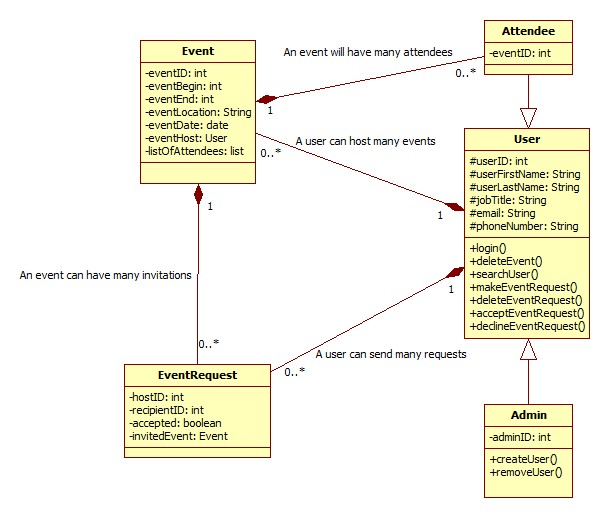
\includegraphics[width=0.75\paperwidth]{ClassDiagram.jpg}} %TODO: Check this sizing at the end.
    \caption{Class Diagram}
    \label{fig:class}
\end{figure}

\subsubsection{Notes}
\textbf{The Classes}
The class diagram consists of four main classes:
\begin{itemize}
    \item \textbf{User:} The user will do the majority of the operations involving the other classes and will allow for event creation and deletion as well as sending, receiving and accepting invitations. The variables inside this class are protected as the class Admin will inherit from this class and an admin must have all the functionality of user and more.
    \item \textbf{Attendee:} A problem we faced was distinguishing between a host and an attendee when creating events. We solved this by having two separate classes to be able to tell between hosts and attendees. An attendee is a user who is attending an event, and contains the event ID of the event to be attended.
    \item \textbf{Event:} The event class will store the details for a single event. Information such as dates, times and locations will be stored in this class through the use of the database.
    \item \textbf{EventRequest:} The Event Request class allows the User class to send out requests specifying the event being invited to as well as the recipient to the request.
    \item \textbf{Admin:} The administrator Class is a user with special privilages which allow for the creation and removal of new and existing accounts. As the Admin class will extend the User class, it will have all the functionality of a User plus more. This authorization will only be given to a select few.
\end{itemize}

\textbf{The Relationships}
\begin{itemize}
    \item \textbf{User - Event:} The relationship between these classes is composition, as an event can no longer exist without the host who created it. The multiplicity is one-to-many, as the user can create many events.
    \item \textbf{Attendee - Event:} The relationship between attendee and event is to allow the class to distinguish between who is the host of an event, and who is simply an attendee. This is to ensure events are destroyed when host accounts are deleted, but not if attendee accounts are deleted.
    \item \textbf{Attendee - User:} An attendee is a user who is attending an event. The attendee has all the attributes of a user but also contains the event ID for the event he/she is attending.
    \item \textbf{User - EventRequest:} The relationship between these classes is aggregation, as even if the user who send the request is deleted, the request can still exist as it links directly to the event. The multiplicity is one-to-many as a user can send many requests.
    \item \textbf{Event - EventRequest:} The relationship between these classes is composition, as if the event a request points to is removed, any requests relating to it must also be removed. The multiplicity is one-to-many as an event can have many event requests.
    \item \textbf{User - Admin:} The relationship between these classes is generalisation, as the class Admin inherits from the class User. This is to ensure the class Admin has all the functionality of a User class aswell as further behaviour such as being able to create accounts.
\end{itemize}
\section{Database}
\subsection{Documentation}
\subsubsection{Entities}
\underline{\textit{Event:}} \\
This entity will store all the information about the events. The unique ID for the entity is the \textit{Event\_ID} and it will be used to determine an event. The entity can hold all the necessary information such as date duration and location. The event is created by a user so the \textit{Host\_ID} is used to identify the user that create the event. The option to keep the event private is also available. 

\underline{\textit{Event Request:}} \\
The Event Request entity is used store the information about an event request. The unique ID is the foreign key from the Event entity. It stores the response of user to the request as well as date invited and if the user seen the request or not. 

\underline{\textit{User:}} \\
All the data of a user are store in the User entity. The unique \textit{User\_ID} is used as a primary and is used to log in in to the system with the required password. The basic personal data of the user are also store such as first name, last name, position, email and phone number. An Admin attribute is used to identify if a user is an admin or a normal user. 

\underline{\textit{Attendee:}} \\
The attendee entity holds the information about the attendance of the event. The combination of the two attributes \textit{User\_ID} and \textit{Event\_ID} will give a combine key for the table. 

\subsubsection{Tables}
\begin{table}[ht]
    \caption{Event}
    \centering
    \begin{tabular}{|c|c|c|c|}
        \hline
        Attributes & PK/FK & Data Type & Constraints  \\
        \hline
        Event\_ID & PK & VarChar(10) & Unique, Not Null \\
        \hline
        User\_ID & FK & VarChar(10) & Not Null \\
        \hline
        Host\_ID & & VarChar(10) & Not Null \\
        \hline
        Event\_Description & & VarChar(30) & Not Null \\
        \hline
        Event\_Start\_Date & & Date & Not Null \\
        \hline
        Event\_Duration & & Integer & \\
        \hline
        Room\_No & & VarChar(10) & \\
        \hline
        Location & & VarChar(15) & \\
        \hline
        Private & & Bit & \\
        \hline
        Comment & & VarChar(100) & \\
        \hline
    \end{tabular}
    \label{tab:event}
\end{table}

\begin{table}[ht]
    \caption{Attendee}
    \centering
    \begin{tabular}{|c|c|c|c|}
        \hline
        Attributes & PK/FK & Data Type & Constraints  \\
        \hline
        Event\_ID & FK & VarChar(10) & Unique, Not Null \\
        \hline
        User\_ID & FK & VarChar(10) & Not Null \\
        \hline
    \end{tabular}
    \label{tab:attendee}
\end{table}

\begin{table}[ht]
    \caption{User}
    \centering
    \begin{tabular}{|c|c|c|c|}
        \hline
        Attributes & PK/FK & Data Type & Constraints  \\
        \hline
        User\_ID & PK & VarChar(10) & Unique, Not Null \\
        \hline
        Admin & & Bit & Not Null \\
        \hline
        Password & & VarChar(20) & Not Null \\
        \hline
        First\_Name & & VarChar(15) & Not Null \\
        \hline
        Last\_Name & & VarChar(15) & Not Null \\
        \hline
        Position & & VarChar(30) & \\
        \hline
        Email & & VarChar(30) & \\
        \hline
        Phone\_Number & & VarChar(20) & Not Null \\
        \hline
    \end{tabular}
    \label{tab:user}
\end{table}

\begin{table}[ht] %TODO: Need to fix the vertical positioning of this
    \caption{Event Request}
    \centering
    \begin{tabular}{|c|c|c|c|}
        \hline
        Attributes & PK/FK & Data Type & Constraints  \\
        \hline
        Event\_ID & FK & VarChar(10) & Unique, Not Null \\
        \hline
        Response & & Bit & Not Null \\
        \hline
        Seen & & Bit & Not Null \\
        \hline
        Date\_Invited & & Date & Not Null \\
        \hline
    \end{tabular}
    \label{tab:event_request}
\end{table}

\begin{landscape}
\clearpage
\subsection{Entity Relationship Diagram}
\begin{figure}[!ht] %TODO: Look into making this landscape too
    \centering\makebox[0.9\textwidth]{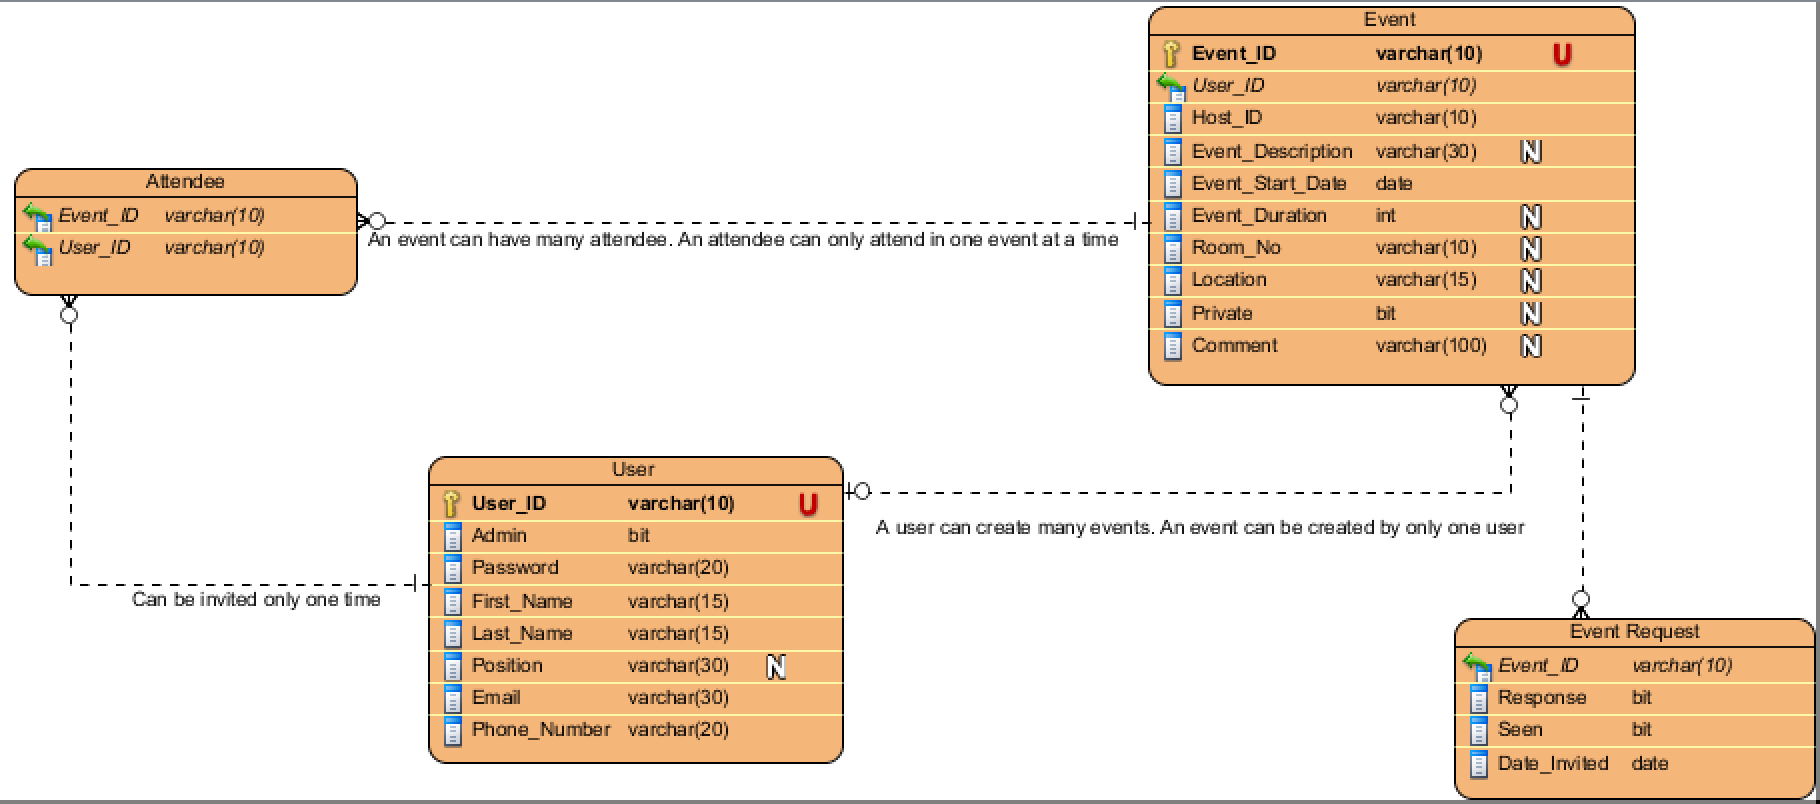
\includegraphics[width=0.75\paperheight]{ERDiagram.png}} %TODO: Check this sizing at the end.
    \caption{Entity Relationship Diagram}
    \label{fig:erd}
\end{figure}
\end{landscape}

\section{Design}
\subsection{High-Level Architecture Diagram}
\begin{figure}[!ht] %TODO: Look into making this landscape too
    \centering\makebox[0.9\textwidth]{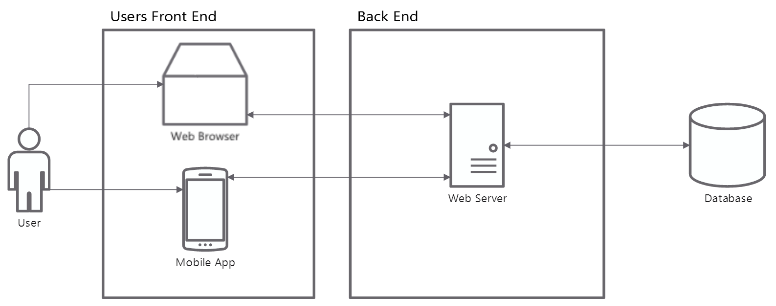
\includegraphics[width=0.75\paperwidth]{ArchDiagram.png}} %TODO: Check this sizing at the end.
    \caption{High-Level Architecture Diagram}
    \label{fig:arch}
\end{figure}

\subsection{Model View Controller}
\subsubsection{Design}
\begin{figure}[!ht] %TODO: Look into making this landscape too
    \centering\makebox[0.9\textwidth]{\includegraphics[width=0.75\paperwidth]{MVCDiagram.png}} %TODO: Check this sizing at the end.
    \caption{MVC Diagram}
    \label{fig:mvc}
\end{figure}

\textbf{Diagram Notes}
The Model-View-Controller design application is made up of several main aspects. It consists of: 
\begin{itemize}
    \item \textbf{The View Classes} \\ 
    Every view in the application will have its own View class. This class handles the updating and gathering of information through the user interface. \\
    \item \textbf{The Controller Classes} \\ 
    Each respective View has its own Controller. This controller class handles communicating the information from the View to the Model class. \\
    \item \textbf{The Model Class} \\ 
    The Model class is where all the respective information will be stored and all logical calculations will take place. This model is shared amongst all controller classes, but its possible that this large Model class will be split up into smaller individual model classes. \\
    \item \textbf{The Server} \\ 
    The Server will handle communications between the database and the Model class. \\
    \item \textbf{The Database} \\ 
    The database is where all the data in the application will be stored using appropriate encryption and hashing depending on the confidentiality of the data stored.
\end{itemize}

\subsubsection{Explanation, Rationale, Benefits and Disadvantages}
The Model-View-Controller (MVC) is a design pattern which focuses on providing a versatile user interface. It separates internal representations of information from the parts of the program which present this information to the user. This section will describe our rationale behind the decision to use the MVC. It will also outline how the use of the MVC design pattern within our application will offer benefits not only to the user, but also to the developers whilst creating the application. Despite this however, its usage also comes with a few disadvantages. These will also be outlined and discussed below.

\textbf{Rationale} \\
The rationale for the use of the MVC pattern within our application is formed from our analysis of the requirements. We needed a design pattern that is both versatile and maintainable whilst remaining uncomplicated to allow other development teams to extend the project in the future. The project needs to be able to perform the basic tasks of a calendar system such as modifying views and updating data. The Model-View-Controller pattern provides the tools to do this in an efficient manner through its relatively simple framework.

\textbf{Benefits} \\
The MVC design pattern comes with a variety of benefits, such as:
\begin{itemize}
    \item \textbf{Separation of Logic and View} \\
    The separate Model and View classes will allow the code for the logic to be separated from the code for the views. This is useful as it promotes good code organisation, making it easier to pinpoint where problems occur and as a result bugs easier to fix. It also allows new features to be implemented more efficiently as well as existing features to be modified effectively. \\
    \item \textbf{Simultaneous Views} \\
    The nature of the MVC's specified encapsulation allows the program to display multiple views based off the same information. This will be useful when we implement the different types of calendars such as the Daily, Monthly and Yearly views. \\
    \item \textbf{Parallel Development} \\
    The loose coupling provided by the MVC pattern will allow separate members of the development team to be working on different aspects of the application at the same time. For example, One member could be working on the logic within the model whilst another on the physical representation of the view to the user. This is an advantage when considering both development speed and team-member co-operation. \\
    \item \textbf{Strong Cohesion} \\
    Whilst the code regarding different aspects of the application will remain separate in different classes, the pattern relies on relationships between these classes, giving the application an essence of strong cohesion. An example of this is how the controller will communicate between the model and the view to perform actions.
\end{itemize}

\textbf{Disadvantages} \\
Whilst the MVC pattern comes with a variety of benefits, it also has several disadvantages. These include:
\begin{itemize}
    \item \textbf{Keeping things Consistent} \\
    As we will be splitting code in to several different classes instead of keeping it form within one class, it will require the maintaining of several classes at once. This can be dangerous as forgetting to update one of these classes could cause bugs and other unforeseen problems. This can be avoided by careful planning and implementation. \\
    \item \textbf{Complexity of Framework and Navigation within Code} \\
    Whilst the MVC provides good organisation and encapsulation, it will require us to adapt the planning steps we made during the planning phase to function correctly with the MVC. This adds new layers of abstraction to the process, making it more complex and difficult to navigate.
\end{itemize}

\section{Appendix}
\subsection{Scenarios}
\includepdf[pages={1}]{scenarios/CI.pdf}
\includepdf[pages={1}]{scenarios/LA.pdf}
\includepdf[pages={1}]{scenarios/BA.pdf}

\clearpage
\subsection{Screen Designs}
\begin{figure}[!ht]
    \centering\makebox[0.75\textwidth]{\includegraphics[width=0.6\paperwidth]{screens/LoginCI.png}} %TODO: Check this sizing at the end.
    \caption{Login - CI}
    \label{fig:login}
\end{figure}

\begin{figure}[!ht] 
    \centering\makebox[0.75\textwidth]{\includegraphics[width=0.75\paperwidth]{screens/GroupCH.png}} %TODO: Check this sizing at the end.
    \caption{Create Group - CH}
    \label{fig:create_group}
\end{figure}

\begin{figure}[!ht]
    \centering\makebox[0.75\textwidth]{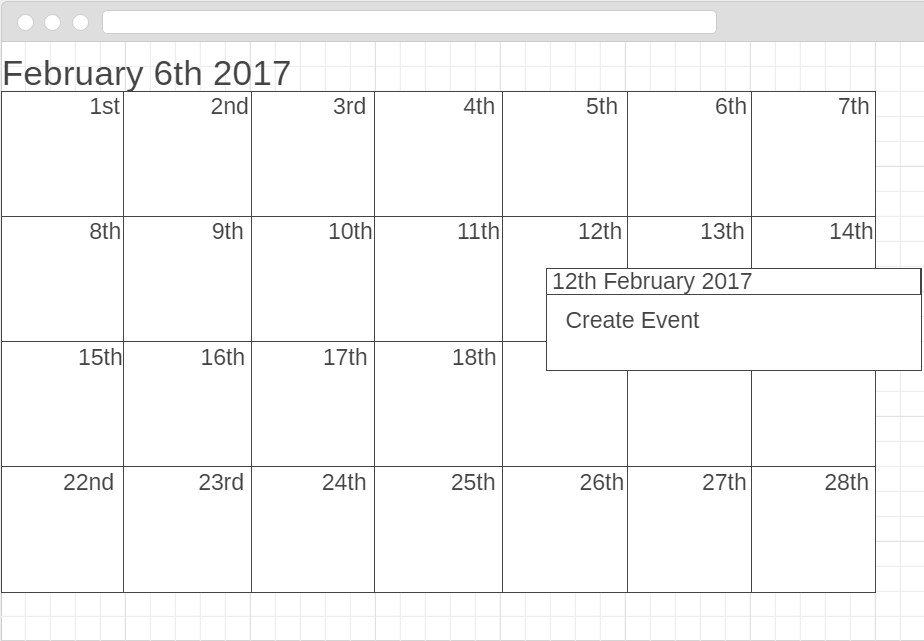
\includegraphics[width=0.75\paperwidth]{screens/CreateEventCalendarLA.png}} %TODO: Check this sizing at the end.
    \caption{Create Group - LA}
    \label{fig:create_event_cal}
\end{figure}

\begin{figure}[!ht]
    \centering\makebox[0.75\textwidth]{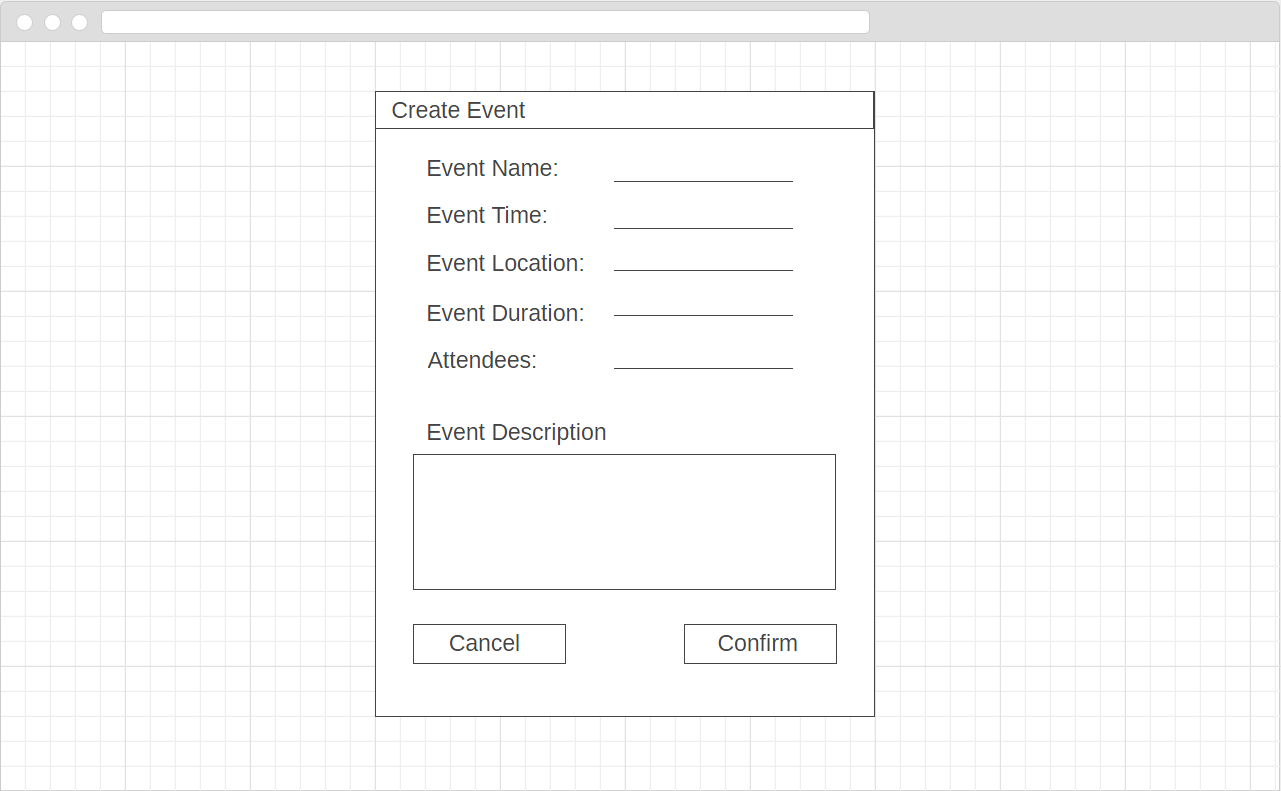
\includegraphics[width=0.75\paperwidth]{screens/CreateEventLA.png}} %TODO: Check this sizing at the end.
    \caption{Create Group - LA}
    \label{fig:create_event}
\end{figure}

\end{document}